\documentclass[12pt]{article}

% Специальный шрифт, чтобы лучше читалось
\usepackage{libertine}

\usepackage{fullpage}

\usepackage{multicol,multirow}
\usepackage{tabularx}
\usepackage{graphicx}
\usepackage{ulem}
\usepackage[utf8]{inputenc}
\usepackage[russian]{babel}
\usepackage{amsmath}
\usepackage{amssymb}

\usepackage{titlesec}

\titleformat{\section}
  {\normalfont\Large\bfseries}{\thesection.}{0.3em}{}

\titleformat{\subsection}
  {\normalfont\large\bfseries}{\thesubsection.}{0.3em}{}

\titlespacing{\section}{0pt}{*2}{*2}
\titlespacing{\subsection}{0pt}{*1}{*1}
\titlespacing{\subsubsection}{0pt}{*0}{*0}
\usepackage{listings}
\lstloadlanguages{Lisp}
\lstset{extendedchars=false,
	breaklines=true,
	breakatwhitespace=true,
	keepspaces = true,
	tabsize=8
}
\begin{document}

\section*{Отчет по лабораторной работе № 5 \\
по курсу \guillemotleft Функциональное программирование\guillemotright}
\begin{flushright}
Студент группы М8О-307-19 МАИ \textit{Ежов Никита Павлович}, \textnumero 9 по списку \\
\makebox[7cm]{Контакты: {\tt nikita.ejov2012@yandex.ru} \hfill} \\
\makebox[7cm]{Работа выполнена: 25.05.2022 \hfill} \\
\ \\
Преподаватель: Иванов Дмитрий Анатольевич, доц. каф. 806 \\
\makebox[7cm]{Отчет сдан: \hfill} \\
\makebox[7cm]{Итоговая оценка: \hfill} \\
\makebox[7cm]{Подпись преподавателя: \hfill} \\

\end{flushright}

\section{Тема работы}
Последовательности, массивы и управляющие конструкции Common Lisp.

\section{Цель работы}
Научиться определять простейшие классы, порождать экземпляры классов, считывать и изменять значения слотов, научиться определять обобщённые функции и методы.


\section{Задание (вариант № 5.27)}
Даны три точки (радиус-вектора), которые могут быть заданы как декартовыми координатами (экземплярами cart), так и полярными (экземплярами polar).

Задание: Определить обычную функцию, возвращающая четвёртую точку такую, что все четыре точки задают параллелограмм.

Результирующая вершина должна быть получена в декартовых координатах - в виде экземпляра класса cart.

(defvar *tolerance* 0.001)

(defun fourth-vertex-cart (v1 v2 v3)
  ...)

\section{Оборудование студента}
Процессор Intel i7-4770 (8) @ 3.9GHz, память: 16 Gb, разрядность системы: 64.

\section{Программное обеспечение}
ОС Kubuntu 20.04.4 LTS, комилятор GNU CLISP 2.49.92, текстовый редактор Visual Studio Code 1.67.1

\pagebreak
\section{Идея, метод, алгоритм}
Идея крайне проста – к точке c3 нужно прибавить вектор, равный разности радиус
векторов точек c2 и c1.

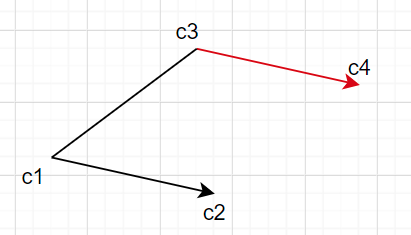
\includegraphics[scale=0.8]{./ris1.png}

\section{Сценарий выполнения работы}
Проще всего воспользоваться предоставленными определениями классов polar и cart,
функциями для вывода, приведения точек из декартовых координат в полярные и об-
ратно, а так же для сложения точек. После этого, для окончательного выполнения ра-
боты, требуется создать оператор вычитания точек и непосредственно саму функцию
для нахождения последней точки параллелограмма.

\section{Распечатка программы и её результаты}

\subsection{Исходный код}
\lstinputlisting{./Ezhov_307_Lab5.lisp}

\pagebreak
\subsection{Результаты работы}
\lstinputlisting{./log5.txt}

\pagebreak
\section{Дневник отладки}
\begin{tabular}{|p{50pt}|p{140pt}|p{140pt}|p{80pt}|}
\hline
Дата & Событие & Действие по исправлению & Примечание \\
\hline
\end{tabular}

\section{Замечания автора по существу работы}

Это первая работу в данном курсе, в которой мне потребовалось проводить исследование не только лишь средств языка Common Lisp.

\section{Выводы}
Я познакомился с обобщёнными функциями, методами и классами объектов в Common Lisp. Описание классов напомнило язык C\#, где 
нужно описывать getter и setter для полей. До этого я не использовал ООП вместе с функциональной парадигмой, в целом, я не 
заметил ощутимой разницу между ООП на Common Lisp и другими языками (не функциональными).

\end{document}
